\documentclass[preprint,12pt,a4paper]{elsarticle}
\usepackage{amsmath,amssymb,booktabs,tabularx,tikz,hyperref,placeins,array}
\hypersetup{hidelinks,pdfauthor={Author names pending}}
\setlength{\emergencystretch}{1em}
\usetikzlibrary{arrows.meta,positioning}
\journal{Science of Computer Programming}
\newcommand{\SourceRevision}{dd97af2ac714f8c0dbf5ddb63ac29cbdb4a2d0dc}
% OrchLang-source-revision: dd97af2ac714f8c0dbf5ddb63ac29cbdb4a2d0dc
\renewcommand{\today}{14 October 2026}
\makeatletter
\def\ps@pprintTitle{%
  \let\@oddhead\@empty\let\@evenhead\@empty
  \def\@oddfoot{\footnotesize\itshape Draft for Science of Computer Programming\hfill\@date}%
  \let\@evenfoot\@oddfoot}
\makeatother
\begin{document}
\begin{frontmatter}
\title{OrchLang: Replayable Verification of Declared LLM Usage Observations}
\author{Author names pending\corref{cor1}}
\address{Affiliations and postal addresses pending}
\cortext[cor1]{Correspondence pending. Author placeholders retained by request; this research draft has not been submitted.}
\begin{abstract}
Equal resource budgets do not establish confidentiality of resource observations. OrchLang is research software for request analysis and conditional usage-law verification in language-model workflows. It combines a bounded compiler, request graphs, rational outcome models and independent certificate replay. Shared-prefix construction and replay resolve a resource limit at 128 calls per secret arm in a controlled family; diagnostics preserve unknown outcomes. A machine-checked theorem covers request-history and local-result agreement for a normalized straight-line fragment under an atomic-read premise. A frozen external-source study retains 59 original candidate files across 12 repositories, with none admitted by the narrow Python frontend. The contribution is an inspectable specialization of established relational and automata methods, with measured software evidence and explicit source, observer and provider boundaries.
\end{abstract}
\begin{keyword}
research software \sep relational verification \sep LLM workflows \sep usage observations \sep reproducibility
\end{keyword}
\end{frontmatter}

\section{Motivation and significance}
An observer who knows the public context can learn from an execution's call count, input usage, output usage or stop position. Equal worst-case caps do not ensure equal distributions of these observations. Conversely, different requests can have the same usage law in a specified model. OrchLang lets researchers distinguish these questions and inspect the assumptions supporting a result.

Resource-aware information flow and relational cost analysis are established techniques~\cite{constant,relcost}. Probabilistic-automata equivalence also predates this software~\cite{kiefer}. PPDL models uncertain multi-call LLM flows~\cite{ppdl}; Agentproof extracts workflow graphs and checks structural and temporal policies~\cite{agentproof}. Recent agent IFC systems address disclosure through tool interfaces~\cite{appa,flowseal}, while ProMCP profiles token and latency costs~\cite{promcp}. OrchLang specializes request identity and a declared usage observer, rather than claiming a new general algorithm or complete agent confidentiality. Prompt-cache timing is a concrete observer outside its model~\cite{cache}.

\section{Software description}
\subsection{Architecture and functionality}
The C++17 compiler checks typed inputs, resolved model contracts, flow policies, literal-bounded retries and conditional token bounds. A bridge exports its admitted request/control fragment. A separate Python frontend accepts a documented static LangGraph subset; unsupported statements, effects, reducers and parallel edges reject. Direct graph JSON supports productive cycles as finite-prefix properties. Assignment invalidates stale result relations, and request comparison retains exact templates, ordered typed arguments and corresponding prior results.

\begin{figure}[ht]
\centering
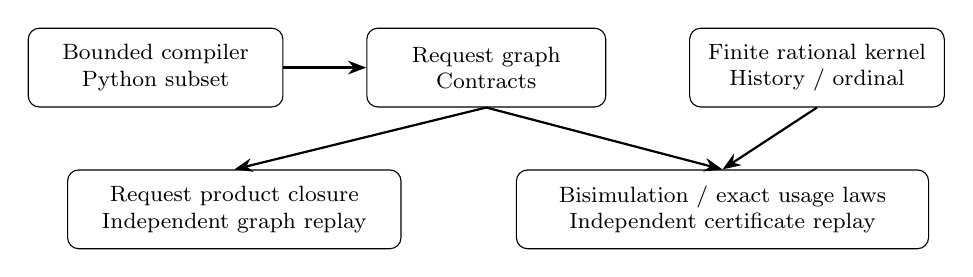
\begin{tikzpicture}[box/.style={draw,rounded corners,align=center,font=\footnotesize,minimum height=1cm,execute at begin node={\hyphenpenalty=10000\exhyphenpenalty=10000}},arr/.style={-{Stealth},thick}]
\node[box,text width=3cm] (src) at (0,0) {Bounded compiler\\Python subset};
\node[box,text width=2.8cm] (graph) at (4.2,0) {Request graph\\Contracts};
\node[box,text width=3cm] (kernel) at (8.4,0) {Finite rational kernel\\History / ordinal};
\node[box,text width=4cm] (req) at (1,-1.8) {Request product closure\\Independent graph replay};
\node[box,text width=5cm] (law) at (7.2,-1.8) {Bisimulation / exact usage laws\\Independent certificate replay};
\draw[arr] (src)--(graph);
\draw[arr] (graph.south)--(req.north);
\draw[arr] (graph.south)--(law.north);
\draw[arr] (kernel.south)--(law.north);
\end{tikzpicture}
\caption{Source adapters and model premises remain distinct from independently replayed graph and usage-law evidence.}
\label{fig:architecture}
\end{figure}

The quantitative tools use successful outcomes from an explicit finite rational kernel. For one public store and the supplied secret assignments, call labels contain the normalized contract and integer input/output usage. Stopped and still-callable mass are separate. Strong bisimulation is sufficient; exact trace-law analysis can decide cases it leaves inconclusive. The latter explores the rational span of $\mu A_w$, where $\mu$ is the initial scenario difference and $A_w$ composes observable-label matrices~\cite{kiefer}. Replay separately reconstructs the semantic system and checks basis words, independence, closure and output columns, or a finite distinguishing witness.

\subsection{Source and resource boundaries}
Version 0.5.0rc2 rejects node names reserved by LangGraph 1.2.14~\cite{langgraph} and module functions shadowing \texttt{str}/\texttt{bool} annotations, including Python 3.14's deferred lookup~\cite{annotations}. Its normalized-IR theorem compares node-entry snapshot reads with eager lowered registers: if later requests never read a field already written by a returned-result call, histories and local results agree for every deterministic history/request oracle. Both theorem checks are closed under the global context. AST extraction, final returned states and whole-graph refinement are not mechanized.

Version-2 trace reports attach bounded reason/phase diagnostics and work counters to unknown outcomes, without a partial system or proof. Replay accepts historical version-1 reports. Certificate prefixes are independently reconstructed once in a trie, preserving exact row checks. Adjacency and parsed-row storage are reserved before allocation. The meters estimate deterministic work; they are not RSS guarantees.

\section{Illustrative examples}
The authored \texttt{different\_requests\_equal\_usage} fixture chooses template \texttt{A} or \texttt{B} by a secret bit. Each has modeled input usage one; a declared kernel gives output usage one or two with probability $1/2$ each. Request equality rejects, but usage-law equality proves and replays. This validates a modeled observer choice, not a provider law.

\begin{table}[ht]
\centering\small
\begin{tabular}{p{0.49\linewidth}lll}
\toprule
Authored case & Request & Bisim. & Exact law\\
\midrule
Different requests, equal usage & Reject & Equal & Equal\\
Equal means, distinct laws & Reject & Inconcl. & Unequal\\
Aggregate hides order & Reject & Inconcl. & Unequal\\
\bottomrule
\end{tabular}
\caption{The same fixed graph/kernel inputs are used across checkers. Rejection and inconclusiveness concern sufficient criteria, not proved leakage.}
\label{tab:observers}
\end{table}

For equal means, one output law is $\{1,3\}$ with equal probabilities and the other is always two: total variation is one at horizon one. The order fixture emits $(1,3)$ or $(3,1)$; aggregate total variation is zero, ordered-trace total variation one at horizon two. Across all twelve authored fixtures, request checking accepts three, bisimulation proves five equal, and exact analysis yields six equal/six unequal; all twelve exact results replay.

\section{Evaluation and reproducibility}
The frozen run includes 44 core stages, 112 native cases in each optimized and sanitizer run, 230 Python audit tests, 23 isolated package stages, and 11/22 pinned LangGraph backend/frontend tests. The separate unchanged-source incident extension passes sixteen stages. These are software checks, not proofs of complete implementation correctness or independent human artifact evaluation.

\subsection{Controlled scaling}
Seven symmetric chain sizes (2--256 calls per secret arm) use identical frozen inputs, one warmup and five measured repetitions in separate processes per size. The solver baseline is revision \href{https://github.com/guyoverclocked/orchlang-compiler-design-project/tree/5aa4ebc669a3fbae72d9a605be250624fd0bcbf5}{\texttt{5aa4ebc}}; current inputs are identical. Both versions complete through 64 calls. At 128 the old producer reaches its replay-preflight cap after closure; prefix sharing now produces and independently verifies equality. Both remain unknown at 256, with a diagnosed residual work limit.

At 64, replay median is 138.51 ms before and 87.51 ms after (36.8\% lower in this run). Reported replay meters are 9,972,749 and 1,784,025 bytes. The new meter additionally charges retained parsed-row storage; these values are not measured memory. Current 128-call medians are 82.79 ms for analysis and 318.68 ms for replay; no old replay-time comparison exists because no certificate was emitted. Timers exclude imports, RSS includes runtime startup, and raw min/max samples, certificate sizes and memory plots are archived. One synthetic family establishes neither broad scalability nor lower memory use.

\subsection{External source and measurement}
A protocol frozen before admission outcomes selected twelve repositories using GitHub search and reported SPDX identifiers. A post-freeze audit against SPDX 3.29.0 OSI flags confirmed the manual allowlist and ordered cohort. A repository-root path-enumeration clarification was logged after outcomes; sources and denominators were unchanged. Enumeration retained 4,348 Python paths, 59 AST-selected candidate files from nine repositories, and one separately recorded non-candidate parse error. All 59 originals are unsupported by the evaluated grammar; no external-source differential ran. First rejections comprise 34 unsupported imports, 19 top-level import statements, four annotation forms and two top-level conditionals. This convenience sample includes tutorials and infrastructure-like files; it provides no prevalence estimate or broad framework-coverage claim.

A separate pinned incident-triage integration executes 22 unchanged-source offline cases and 45 mock calls. Its controlled shared-meter witness has 456 unique estimated usage units but 687 when returned snapshots are summed. A bounded isolation wrapper and replay reproduce that source-specific finding; they do not prove general concurrency safety. Local \texttt{tiktoken} 0.12.0~\cite{tiktoken} calibration on 90 paired call texts and twelve authored controls distinguishes character estimates from three BPE counts. No provider envelopes, cache discounts, usage invoices or stochastic provider premises are validated.

\begin{table}[ht]
\centering\footnotesize
\begin{tabular}{@{}p{0.045\linewidth}>{\raggedright\arraybackslash}p{0.30\linewidth}>{\raggedright\arraybackslash}p{0.59\linewidth}@{}}
\toprule
 & Code metadata description & Metadata\\
\midrule
C1 & Current code version & 0.5.0rc2 research candidate\\
C2 & Permanent link to code/repository used for this code version & \href{https://github.com/guyoverclocked/orchlang-compiler-design-project/tree/\SourceRevision}{\texttt{\SourceRevision}}\\
C3 & Permanent link to Reproducible Capsule & Hash-bound source/evidence archives prepared; persistent capsule identifier pending\\
C4 & Legal Code License & MIT; upstream snapshot licenses retained\\
C5 & Code versioning system used & Git\\
C6 & Software code languages, tools, and services used & C++17; Python 3.10+ core; optional LangGraph; Rocq 9.3.0 proof check\\
C7 & Compilation requirements, operating environments and dependencies & macOS recorded run; make/C++17 and Python; optional locked LangGraph, tokenizer and plotting environments\\
C8 & If available, link to developer documentation/manual & \href{https://github.com/guyoverclocked/orchlang-compiler-design-project/blob/\SourceRevision/docs/PUBLICATION_UPGRADE.md}{Publication reproduction guide} and \href{https://github.com/guyoverclocked/orchlang-compiler-design-project/tree/\SourceRevision/docs}{developer documentation}\\
C9 & Support email for questions & Author email pending; \href{https://github.com/guyoverclocked/orchlang-compiler-design-project/issues}{public issue tracker}\\
\bottomrule
\end{tabular}
\caption{Software metadata. Code identity is distinct from the later paper/evidence commit. Author fields remain explicit placeholders.}
\end{table}
\FloatBarrier

\section{Impact and limitations}
The software provides eight installed analysis and replay commands, exact witnesses and explicit unknown outcomes for workflow usage research. External adoption is unmeasured. Current source adapters are narrow. Broader source support, refinement of complete programs, error and retry models, provider accounting and independent human reproduction remain necessary extensions. Usage-law equality excludes output content, timing, transport and persistent-store privacy; it does not establish termination or whole-cycle budgets.

\section*{Declarations and software availability}
Author identities, affiliations, correspondence, CRediT, funding and competing interests await author completion. Codex and GPT-6 Luna agents assisted research, implementation, tests, proof and drafting. Final human review and responsibility have not been asserted. This draft has not been submitted. The declared software revision includes every named source study; fresh evidence and the companion paper are bound by the publication manifest. Documentation describes one-command reproduction and separate optional environments.



\begingroup\small\raggedright
\setlength{\bibsep}{3pt}
\begin{thebibliography}{12}
\bibitem{constant} V.C. Ngo et al., Verifying and Synthesizing Constant-Resource Implementations with Types, IEEE S\&P (2017). \href{https://doi.org/10.1109/SP.2017.53}{doi:10.1109/SP.2017.53}.
\bibitem{relcost} E. \c{C}i\c{c}ek et al., Relational Cost Analysis, POPL (2017). \href{https://doi.org/10.1145/3009837.3009858}{doi:10.1145/3009837.3009858}.
\bibitem{kiefer} S. Kiefer et al., Language Equivalence for Probabilistic Automata, CAV (2011), 526--540. \href{https://doi.org/10.1007/978-3-642-22110-1_42}{doi:10.1007/978-3-642-22110-1\_42}.
\bibitem{ppdl} L. Mandel et al., PPDL: LLM-Based Flows as Probabilistic Programs, ICML, PMLR 306 (2026). \href{https://proceedings.mlr.press/v306/mandel26a.html}{Proceedings}.
\bibitem{agentproof} M. Xavier et al., Agentproof: Static Verification of Agent Workflow Graphs, \href{https://arxiv.org/abs/2603.20356v1}{arXiv:2603.20356v1} (2026), preprint.
\bibitem{appa} A. Kravchenko et al., APPA: Recoverable Information-Flow Control for Real-World LLM Agents, \href{https://arxiv.org/abs/2607.24625v2}{arXiv:2607.24625v2} (2026), preprint.
\bibitem{flowseal} M. Shim et al., Confuse the Model, Control the Flow: Understanding and Mitigating Privacy Leakage from LLM Agents with Information Flow Control, \href{https://arxiv.org/abs/2609.14003v1}{arXiv:2609.14003v1} (2026), preprint.
\bibitem{promcp} S. Anjum et al., ProMCP: Profiling Token Flows and Latency Costs in Model Context Protocol-Based LLM Agents, Findings of ACL (2026). \href{https://doi.org/10.18653/v1/2026.findings-acl.1967}{doi:10.18653/v1/2026.findings-acl.1967}.
\bibitem{cache} C. Gu et al., Auditing Prompt Caching in Language Model APIs, ICML, PMLR 267 (2025). \href{https://proceedings.mlr.press/v267/gu25b.html}{Proceedings}.
\bibitem{langgraph} LangChain, LangGraph 1.2.14, tagged implementation. \href{https://github.com/langchain-ai/langgraph/blob/1.2.14/libs/langgraph/langgraph/graph/state.py}{StateGraph source}.
\bibitem{annotations} L. Hastings, PEP 649: Deferred Evaluation of Annotations Using Descriptors. \href{https://peps.python.org/pep-0649/}{Python enhancement proposal}.
\bibitem{tiktoken} OpenAI, tiktoken 0.12.0, software release. \href{https://github.com/openai/tiktoken/releases/tag/0.12.0}{Tagged release}.
\end{thebibliography}
\endgroup
\end{document}
